\section{Introduction}
A state of forced migration exists when a significant number of people are displaced due to socio-political issues, armed conflicts, human-made or natural disasters. This research focuses on the role of violence and security threats in forced migration. Tracking and predicting population displacement is a critical step in developing an early warning system in the humanitarian crisis. Furthermore, the development of events in conflict regions influences the decision to move and thus to detect displacement signals is essential for studying forced migration. To capture these events, news articles are a powerful source.

However, building a quantitative model that extracts and measures the forced migration signals (particularly violence in this research) and finds the relationship between violence and forced displacement remains relatively unexplored. To contribute to this problem, we introduce the PD-SEF framework\footnote{Code for this project is available on https://github.com/YorkUIRLab/eosdb} to detect signals of forced population displacement by analyzing news articles. We mainly focus on Iraq and Syria as case studies and our experiments are centered around detecting violence as the most critical indicator of forced migration. 

The main contribution of this paper is to propose a comprehensive framework for analyzing a large news corpus and extract the signals that trigger forced population displacement. Furthermore, a displacement prediction model is devised to take these signals into account and estimate the future population movements. 

The experimental results show the improvement of our extracted violence scores over the previous state-of-the-art methods and validate our assumption that violence is an effective feature for building prediction models for forced migration. 

\section{Related work}
\subsection{Detecting Factors of Forced Migration}
In 1997, Schmeidl \cite{schmeidl1997exploring} developed a theoretical model of refugee migration based on the factors with estimated magnitude. These factors include economical under-development, human rights violation, ethnic and civil conflicts. These factors were then included in a pooled time-series analysis to predict the number of refugees. This research showed that economic and intervening policy variables are less useful for predicting refugee migration than the threat of violence. This work is different from our model regarding the methodology used for extracting the forced migration signals. Unlike this research that uses manually generated scores from various resources for the factors mentioned above, we automatically extract the score of the factors of forced migration from news articles.

To analyze the trends of a particular topic over time, Wang et. al. introduced Topics over Time (TOT), which is an LDA-based topic model \cite{Wang2006}. To achieve this, they jointly model word co-occurrences and localization in continuous time windows. Furthermore, time-sensitive document topic modeling was proposed in [2], where the policies of the European Parliament (EP) are studied through dynamic topic modeling of the documents generated by the parliaments (e.g. debates and bills). Political agenda of the EP has evolved significantly over time as new events and topics unfold. 

The most similar research to ours was performed by Agrawal et al.\cite{agrawal2016detecting}. They introduced a method to extract the magnitude of violence from news articles. This method uses word embedding techniques to embed the words of news articles and then uses similarity measures within the embedding space to compute the similarity between the words of a document and a set of predefined seed words indicating violence. At last, a correlation was observed between the extracted violence scores and the number of migrated people. This work only detects the magnitude of violence from news articles and does not focus on other factors of forced migration. The quality of the extracted violence scores considerably depends on the quality of the manually generated set of seed words.

\subsection{Topic Modeling}
Topic modeling is an effective method to process large amount documents. The method allows for discovery of a distinct set of topics among the corpus. A topic modeling approach can connect the words with similar meaning and form topics.

\subsubsection{LDA (Latent Dirichlet Allocation)}
LDA belongs to the group of generative probabilistic models for documents. Based on an intuitive idea that each document is comprised of a mixture of topics, and each topic is a discrete probability distribution of how likely each word is to appear on a given topic. Given set of documents $W = \{w_1, w_2, ...,  w_d\}$, to generate a word token $w_n$  from document d, a discrete topic assignment $z_n$ is drawn from a document-specific distribution over the T topics $\theta_d$. This value is drawn from a Dirichlet prior with hyper-parameter $\alpha$. The inference task in topic models is defined as inferring the document proportions $\{\theta_1, ... \theta_D\}$ and the topic-specific distributions $\{\phi_1, ... ,  \phi_T\}$ \cite{Mimno}. 
Building on foundations of LDA, \cite{Griffiths} proposed using a Dirichlet prior on topic-word distribution $\phi$, with additional hyper-parameter $\beta$. Further, \cite{Griffiths} used collapsed Gibbs sampling to estimate the topic space distribution indirectly. This method iteratively estimates the probability assignment of each word to the topics, conditioned on the current topic assignment of all other words. The popular topic modeling toolkit MALLET is based on LDA with Gibbs sampling.


\section{OUR PROPOSED FRAMEWORK}
The PD-SEF framework consists of three components. The first component includes analyzing a large corpus of news articles using topic modeling techniques in order to provide an efficient and compact representation. The dimensionality reduction achieved by topic modeling is an important benefit for the second component where human knowledge is needed to analyze the extracted topics. The second component uses the extracted topics to output a degree of violence for each month, which is then used in the third component to build prediction models for forecasting the future number of refugees from Syria and Iraq.


\subsection{Topic Modeling}

\subsubsection{Non-negative Matrix Factorization (NMF)} 
Matrix factorization is a widely used approach for the analysis of high-dimensional data. The objective of NMF is to extract meaningful features from a set of non-negative sparse vectors. The NMF is successfully applied to different applications, such as image processing, hyper-spectral imaging,  and text mining.  Here we focus on the property of NMF to identify topics in a given set of documents and classify the documents among the underlying topics.

Let each column of the non-negative data matrix $X \in \mathbb{R}$ represents a document and each row to a word in the dictionary. In this matrix, the $(i, j)^{th}$ entry corresponds to a number of times the $i^{th}$ word appears in the $j^{th}$ document. Each column of the matrix X is the word count of a $j^{th}$ document. In practice, the bag-of-word is replaced by term frequency - inverse document frequency (TF-IDF) representation of the document. The use of TF-IDF pre-processing has shown to help results of NMF by down-weighting the contribution of high-frequency terms while boosting the effect of rarer terms in the corpus \cite{Greene2016,Gillis2014}. The matrix X is rather sparse since most of the documents only have a small subset of the dictionary terms.

Given matrix X and factorization rank $r$, NMF decomposition generates two non-negative factors W and H, where $X \approx W H$ (Eq. \ref{eq:nfm}) \cite{Lee1999}. 

\begin{multline}\label{eq:nfm}
\underbrace{X(:,j)}_\text{$j^{th}$ document.} \approx \sum_{k=1}^{r} \underbrace{W(:,k)}_\text{$k^{th}$ topic.} \underbrace{H(k,j)}_\text{ weight of $k^{th}$ topic in $j^{th}$ document.} , \\
with W \geq 0 and H \geq 0.
\end{multline}

The results NMF decomposition can be interpreted by examining the W and H matrix. Because W is non-negative, each column of W can also be interpreted as a bag-of-words representation of the document.

\begin{figure}[t]
\centering

\includegraphics[scale=.4]{img/NMF}
\label{fig:NMF}
\caption{NMF factorization}
\end{figure}

At the same time, since weights in linear combinations are also non-negative, $H \geq 0$, the union with sets of words in W can approximate the original document. Since the number of documents (columns in X) is much larger than a number of basis elements (columns in W), the elements of W contains the set of words found simultaneously appearing in multiple documents. The weights in linear combinations, matrix H, assign the documents to different topics. Therefore, NMF  can identify the topics across the documents and classify each document according to the topics it belongs to. Inspired by the work done in \cite{Greene2016} to extract dynamic topics, we apply NMF on time-windows of news media corpus to extract the evolving topics.

\textbf{Topic model generation:}
The first step in topic modeling is to divide the news corpus into monthly time windows. In this step, the news articles are processed and labeled according to their timestamps. The length of the time windows can be a day, week or month. The time windows can have effects on the granularity of the topics generated. In this framework, we chose the monthly time window for the topic analysis. 

After generating time windows, we start by generating topic models for each time window. All documents in the time window are processed and passed to the topic modeling algorithm. Topic modeling falls under the unsupervised learning and needs parameter tuning. The most critical parameter in topic modeling is the number of topics $k$. Topic models are susceptible to the number of topics, and the quality of the topics generated varies drastically if $k$ is not selected correctly. To identify the optimal topic number $k$, we generate topic models with the number of topics in the range of $k \in \{10, 50\}$ with an increment of two.




\textbf{Topic model coherence analysis:}

To find the optimal topic number, we apply topic coherence measures to choose the best result. Here, we apply two different topic coherence measures. Quantifying the coherence of the topics extracted from topic modeling methods is a crucial part of this research. The primary concern about the efficiency of the statistical topic modeling is the presence of weak and obscure topics in the results. Topics with mixed and loosely related concepts usually fail to generate meaningful insight for the users. As Mimno et. al. \cite{Mimno} observed, there is a strong relationship between the number of topics and quality of the topics judged by domain experts. This is because as the number of topics increases, the quality of word distribution constituting the topic decreases. At the same time, the lower number of topics may result in an undesirable generalization of topic distribution in the corpus.  

Recent work on the evaluation of statistical topic models have focused on topic's semantic coherence \cite{Ocallaghan,Roder2015}. To calculate the topic coherence score, we use TC-W2V \cite{Ocallaghan} and Unify framework \cite{Roder2015}. We choose the topic model with the highest coherence to generate the window topic documents. 

\begin{figure}[!ht]
\centering
\caption{Topic generation process}

\includegraphics[scale=.4]{img/topic_generation}
\label{fig:topicgeneration}
\end{figure}

At this step, we have generated and evaluated the coherence of the topic models for each monthly time window (Fig \ref{fig:topicgeneration}). The topic models are a probability distribution of the words that appear in each topic. For each of the topics, we generate a topic-document to represent the topic. Topic-documents are generated by ranking the top keywords appearing in the topic by their probability of appearing in the topic. The number of topics per time window may vary since we are only using the topics with best coherence score in the range of $k$.

\subsection{Violence Scores Extraction}
The topic-documents generated from component 1 form a new corpus with reduced dimensionality. Our next step is to label a topic document with a category such as violence, relief, economic issues. This step can be done automatically using a topic labeling method. But we did it manually with the help of social scientist to ensure the quality of the topic labels. That is because the quality of the labeled data directly effects the quality of the forced displacement prediction model. The result of this process is a set of labeled monthly topic-documents. 

The violence score for each month is then defined by the total number of violence topics for each month divided by the total number of topics for each month. As we want to model the population movements, we need to measure the impact of violence on people, which causes the movement. The degree of violence somewhat depends on the scale of other events happening at the same time. Thus, we put the division to get a scale of the impact of violence on people.


\subsection{Topic Classification for automatic labeling}
We used the topic modeling results as a way to reduce the dimensionality of the entire news media corpus. The topics, we conjecture, represents the gist of the overall hidden themes in this setting. The classification task of the news articles based on the extracted topics is useful for labeling the incoming news media articles. The effort to sort and classify the violence signals from news media has a temporal aspect. We used different classification techniques to classify extracted topics according to relativity to factors of forced migration, specifically violence in this research. We used the topic documents, the top keywords based on the probability distribution in the topic, as a documents, and used the topic labels (described in Section \ref{topicLabeling}) to train supervised classification task. 

For classification task, we examined  support vector machine classifier (SVM-Linear) \cite{Crammer:2002:AIM:944790.944813}, XGboost\cite{DBLP:journals/corr/ChenG16}, Logistic regression, and Stochastic Gradient Descent.

\subsection{Building Prediction Models}
A three-step procedure is performed to analyze the extracted violence scores and to build prediction models for forced displacement:

\textit{Step 1:}
Extracted violence scores are used as input features of regression models to predict the future number of refugees. This step investigates whether or not the violence scores are adequately effective to make predictions. 

\textit{Step 2:} To compare the extracted violence scores against a baseline feature, we build an auto-regression model on time-series of refugee population displacement. Auto-regression is a regression model with lag variables as input features as it is built based on the assumption that the previous values (called lag variables) might affect the future values. An auto-regression model is built in this step using the previous number of refugees as input features and make predictions relying on no other external source. The lag variable of 1 means the previous observation in time-series (t-1) is used to predict future observation (t). The lag variable of 2 means (t-2) is used to predict (t), and so on. 
This step investigates validity of the assumption that previous movements affect the future displacements and provides a baseline feature for comparing quality of violence scores with.

\textit{Step 3:} Two previous steps are combined by using both violence scores and lag variables as inputs for the predictive regression model. This step investigates the effectiveness of violence scores in improving the accuracy of the prediction model built in step 2.

\section{Experimental Settings}

\subsection{Datasets}
\textit{EOS dataset:}
The Expanded Open Source (EOS)\footnote{https://osvpr.georgetown.edu/eos} dataset, maintained by Georgetown University researchers, is a vast unstructured archive of over 700 million news articles. The news articles used in this research are filtered based on relativity to Iraq and Syria using the EOS search engine. The initial filtering helps to have a more focused, and smaller news set. The corpus consists of 680,456 news articles spanning from January 2012 to June 2017. Figure \ref{fig:corpus_histogram} describes the document length characteristics of the data used for this experiment.

\begin{figure}[t]
\caption{EOS data set statistics.}
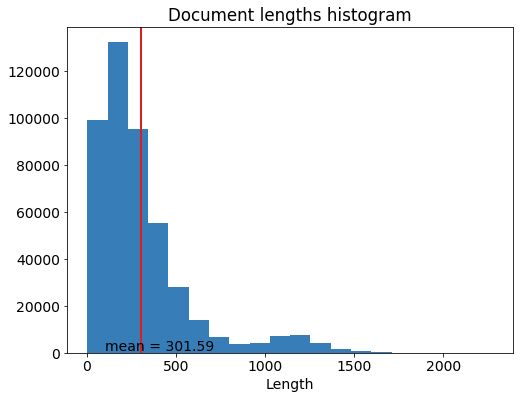
\includegraphics[scale=.35]{img/corpus_histogram.png}
\centering
\label{fig:corpus_histogram}
\end{figure}

\textit{UNHCR dataset:}
We used UNHCR\footnote{United Nations High Commissioner for Refugees} Refugee population statistics dataset to capture the number of refugees on a monthly basis. For building prediction models we focus on a subset of UNHCR dataset related to Iraqi and Syrian refugees from 2012 to 2017, as EOS dataset provides the news articles for this period of time. As the distributions of Iraqi and Syrian refugees are similar over the time period and we do not have distinguished violence scores for Iraq and Syria, a new time series is made by computing the average of Iraqi and Syrian refugees and is used for all the following experiments. New time series has a mean of 11,080.05 and standard deviation of 11,206.95 with a minimum of 0 and maximum of 48,753.


\subsection{Time Window Collection \& Topic Labeling} \label{topicLabeling}
To analyze the time evolution of topics over the large document collection, we first need to separate the documents into time-stamped bins. Followed by the previous works\cite{Sulo2010}, we divide the EOS data into a set of sequential non-overlapping time windows $\{T_1, ... , T_i\}$. Each time window bin consists of sequentially ordered documents based on the published date. Each bin has a set of non-overlapping documents divided on a monthly basis.

The monthly time window bins ensure that an enough number of documents exist in each bin. The reason for creating time window bins is two-fold: first, we are interested in the topical events in shorter window sizes. Second, the short-lived topics may be obscured by the generalized topics learned from the entire collection. The monthly time window also allows us to identify more granular and short-term topics, as well as generalized topics over longer terms. 

We manually labeled the monthly extracted topics into seven categories of violence/terrorism, economic issues, environmental issues, political issues, religious conflicts, refugee crisis, and relief.

\subsubsection{Classification Baselines}
We compare the performance of our topic classifiers with various traditional baseline methods, including linear methods, SVM and regularized linear models with stochastic gradient descent (SGD) \cite{bottou-2010}.

\subsection{Prediction Models}
We evaluate our prediction models in three settings. Predicting t+1, t+2 and t+3. The Root Mean Square error is reported separately for each time step and the error of the prediction is calculated based on the test dataset.
A walk forward model evaluation is performed when evaluating the prediction results. Each time step in the test set will be given to the model one at a time, the model predicts a value for the given time step and then the actual value for that time step will be accessible to the model to make the next predictions based on it. This is because we have more than 10 instances in our test set and it is not possible to accurately predict all these corresponding values only based on the information available at the present time. Walk forward model evaluation mimics a real world scenario when we make predictions for the next 3 months (t+1,t+2,t+3) and then the information about the next month will be released (in our case news articles and number of refugees) and then this information is used to make predictions for the next upcoming months. 

Training set includes $80\%$ of the data (Jan 2012-Mar 2016) and test set includes the last 20\% observations in UNHCR dataset (May 2016-Apr 2017) which is equal to 12 instances. A total of 36 forecasts will be performed. (12 forecasts for each setting of t+1,t+2,t+3))

\subsubsection{Computation} For this experiments, we used machine with Intel Core i7, and 32 GB of RAM. The processing news text and time window topics took almost 9 hours on this machine. 

\section{Results and Discussion}

\subsection{Prediction Models Evaluation}
Table \ref{predictionModels} reports RMSE of several prediction models in different prediction settings (t+1, t+2, t+3) and steps (with different input features.) For Multi-layer Perceptron regression(MLP), Random Forest, Linear Regression, Support-Vector regression(SVR) and Stochastic gradient descent(SGD) the grid search is used to fine tune the model parameters and report the best results. We also optimized our Neural Network based models by different optimization functions (ADAM, RMSProp). The three neural-network based models are:

\textit{LSTM and GRU models:} 1 input, a hidden layer with 4 LSTM or GRU blocks, an output layer that makes a single value prediction.

\textit{LSTM2LSTM:} 1 input layer is feeding into an LSTM layer with the internal state of size 50, with 0.2 dropout rate and another LSTM layer with the internal state of size 100, which then feeds into a fully connected standard layer of 1 neuron with a linear activation function for prediction.

Considering that UNHCR time series has a mean of 11,080 and standard deviation of 11,206, errors of prediction models are within the tolerance range. The least RMSE for each setting is bold in the table.
Intuitively, predicting t+3 is harder than t+2 which is harder that t+1, because of the more missing data. However, the improvement of step 3 over step 2 is most tangible in t+2. This is justifiable due to the 2-month gap explained in section 5.3. Results show that violence scores are not sufficient to make predictions, however, for 7 out of 8 models, average error decreased when converting from step2 to step3, indicating the effectiveness of both lag variables and violence scores in models' performance. The impact of previous movements on future movements might be due to the effect of the surrounding environment on people.
% \vspace{-1.5em}

\begin{figure}[!ht]
\centering
 \caption{Prediction model performance}
 \label{fig:mlp}
 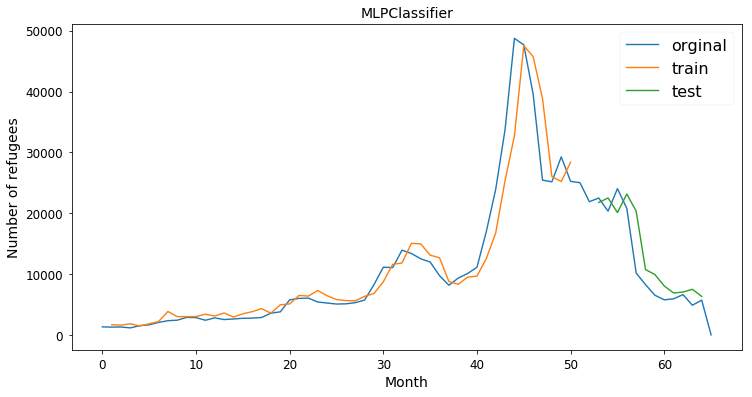
\includegraphics[height=0.5\columnwidth,width=0.9\columnwidth]{img/mlp_step_1}
\end{figure}

Best performance on average is for MLPregression (Fig \ref{fig:mlp}). We believe this success is due to its ability to capture the historical observations through the input window (unlike SGD, SVR and linear regression). Furthermore, it has less complexity compared to LSTM and GRU, making it more suitable for our small dataset.


\begin{table*}[!ht]
\centering
\caption{RMSE of forced displacement prediction models}
\label{predictionModels}
\resizebox{\textwidth}{!}{
% \begin{tabular}{lcccccc}
\begin{tabular}{lclclll}
\toprule
                  & \multicolumn{2}{c}{Input Features}                          & \multicolumn{4}{c}{Predicted Time-Step}                                                                           \\
Regression Models & Lag Variable          & \multicolumn{1}{c}{Violence Scores} & t+1                   & \multicolumn{1}{c}{t+2} & \multicolumn{1}{c}{t+3} & \multicolumn{1}{c}{AVG (t+1,t+2,t+3)} \\ \midrule

                                                                          & \checkmark           & \multicolumn{1}{l}{} & 3,266.05                 & 4,767.52                 & 6,239.41         &     4,757.64   \\
LSTM                                                                      & \multicolumn{1}{l}{} & \checkmark           &9,708.36       &8,959.28         &8,250.36       &8,972.66  \\
                                                                          & \checkmark           & \checkmark           & 3,546.03                 & 4,408.93                 & 4,932.07               & 4,295.67$\downarrow$ \\ \midrule
                                                                          & \checkmark           & \multicolumn{1}{l}{} & 3,266.06                 & 5,151.28                 & 4,094.39               & 4,170.57 \\

LSTM2LSTM                                                       & \multicolumn{1}{l}{} & \checkmark       &    9,563.09           &       8,786.27        &           8,077.21          &  8,808.85 \\
                                                                          & \checkmark           & \checkmark           & \textbf{3,225.44}              & 4,772.04                 & 4,099.56             &  4,032.34$\downarrow$ \\ \midrule
                                                                          & \checkmark           & \multicolumn{1}{l}{} & 3,955.5                  & 4,674.38                 & 4,339.82              &  4,323.23 \\

GRU                                                                       & \multicolumn{1}{l}{} & \checkmark           &           9,706.84        &       8,960.13         &       8,251.46     &   8,972.81 \\
                                                                          & \checkmark           & \checkmark           & 3,865.65                 & 4,467.03                 & 4,283.05              &  4,205.24$\downarrow$\\ \midrule
                                                                          & \checkmark           & \multicolumn{1}{l}{} & 4,663.21                 & 3,599.11                 & 3,996.31              &  4,086.21 \\

MLP  & \multicolumn{1}{l}{} & \checkmark           &         5,129.4       &          4,875.94       &      4,809.29      & 4,938.21  \\
                                                                          & \checkmark           & \checkmark           & 3,664.41                 & \textbf{3,343.65}                 & \textbf{3,995.79}              &  \textbf{3,667.95}$\downarrow$ \\ \midrule
                                                                          & \checkmark           & \multicolumn{1}{l}{} & 7,987.04                 & 8,804.43                 & 9,477.96              &  8,756.47 \\

Random Forest              & \multicolumn{1}{l}{} & \checkmark           &        11,133.63       &       7,721.94            &      7,137.77     &  8,664.44 \\
                                                                          & \checkmark           & \checkmark           & 6,902.37                 & 7,622.25                 & 9,505.81             &   8,010.14$\downarrow$ \\ \midrule
                                                                          & \checkmark           & \multicolumn{1}{l}{} & 3,550.41                 & 3,645.06                 & 4,033.56             &   3,743.01 \\

Linear Regression                                                        & \multicolumn{1}{l}{} & \checkmark           &               6,734.52       &       7,122.58        &         7,297.1       &   7,051.4 \\
                                                                          & \checkmark           & \checkmark           & 3,658.19                 & 3,506.19                 & 3,997.17             &  3,720.51$\downarrow$ \\ \midrule
                                                                          & \checkmark           & \multicolumn{1}{l}{} & 5,074.14                 & 5,243.61                 & 5,391.58               & 5,236.44 \\

SVR                       & \multicolumn{1}{l}{} & \checkmark           &       6,652.57     &      5,972.41       &     5,324.02       &  5,983.0 \\
                                                                          & \checkmark           & \checkmark           & 4,898.5                  & 4,928.62                 & 4,729.99              &  4,852.37$\downarrow$ \\ \midrule
                                                                          & \checkmark           & \multicolumn{1}{l}{} & 3,526.84                 & 4,387.69                 & 5,239.25              &  4,330.53 \\

SGD Regression                               & \multicolumn{1}{l}{} & \checkmark           &        6,655.03      &   7,060.31      &       6,939.52       &   6,884.95 \\
                                                                          & \checkmark           & \checkmark           & 3,956.09                 & 4,833.23                 & 4,632.28              &  4,473.86$\uparrow$\\ 
 \bottomrule
\end{tabular}
}
\end{table*}


\subsection{Violence Scores Evaluation}
To evaluate PD-SEF violence scores and to compare them with violence scores extracted from EOS articles using the method introduced in \cite{agrawal2016detecting}, we compare both sets of scores against UNHCR dataset and check for Pearson correlation between violence scores and number of refugees. The PD-SEF violence showed 22\% more correlation with refugee displacement than violence scores of \cite{agrawal2016detecting}.

\begin{figure}[!ht]
\centering
  \caption{Scaled violence scores vs. average displacement}
  \vspace{0em}
  \label{fig:ours}
  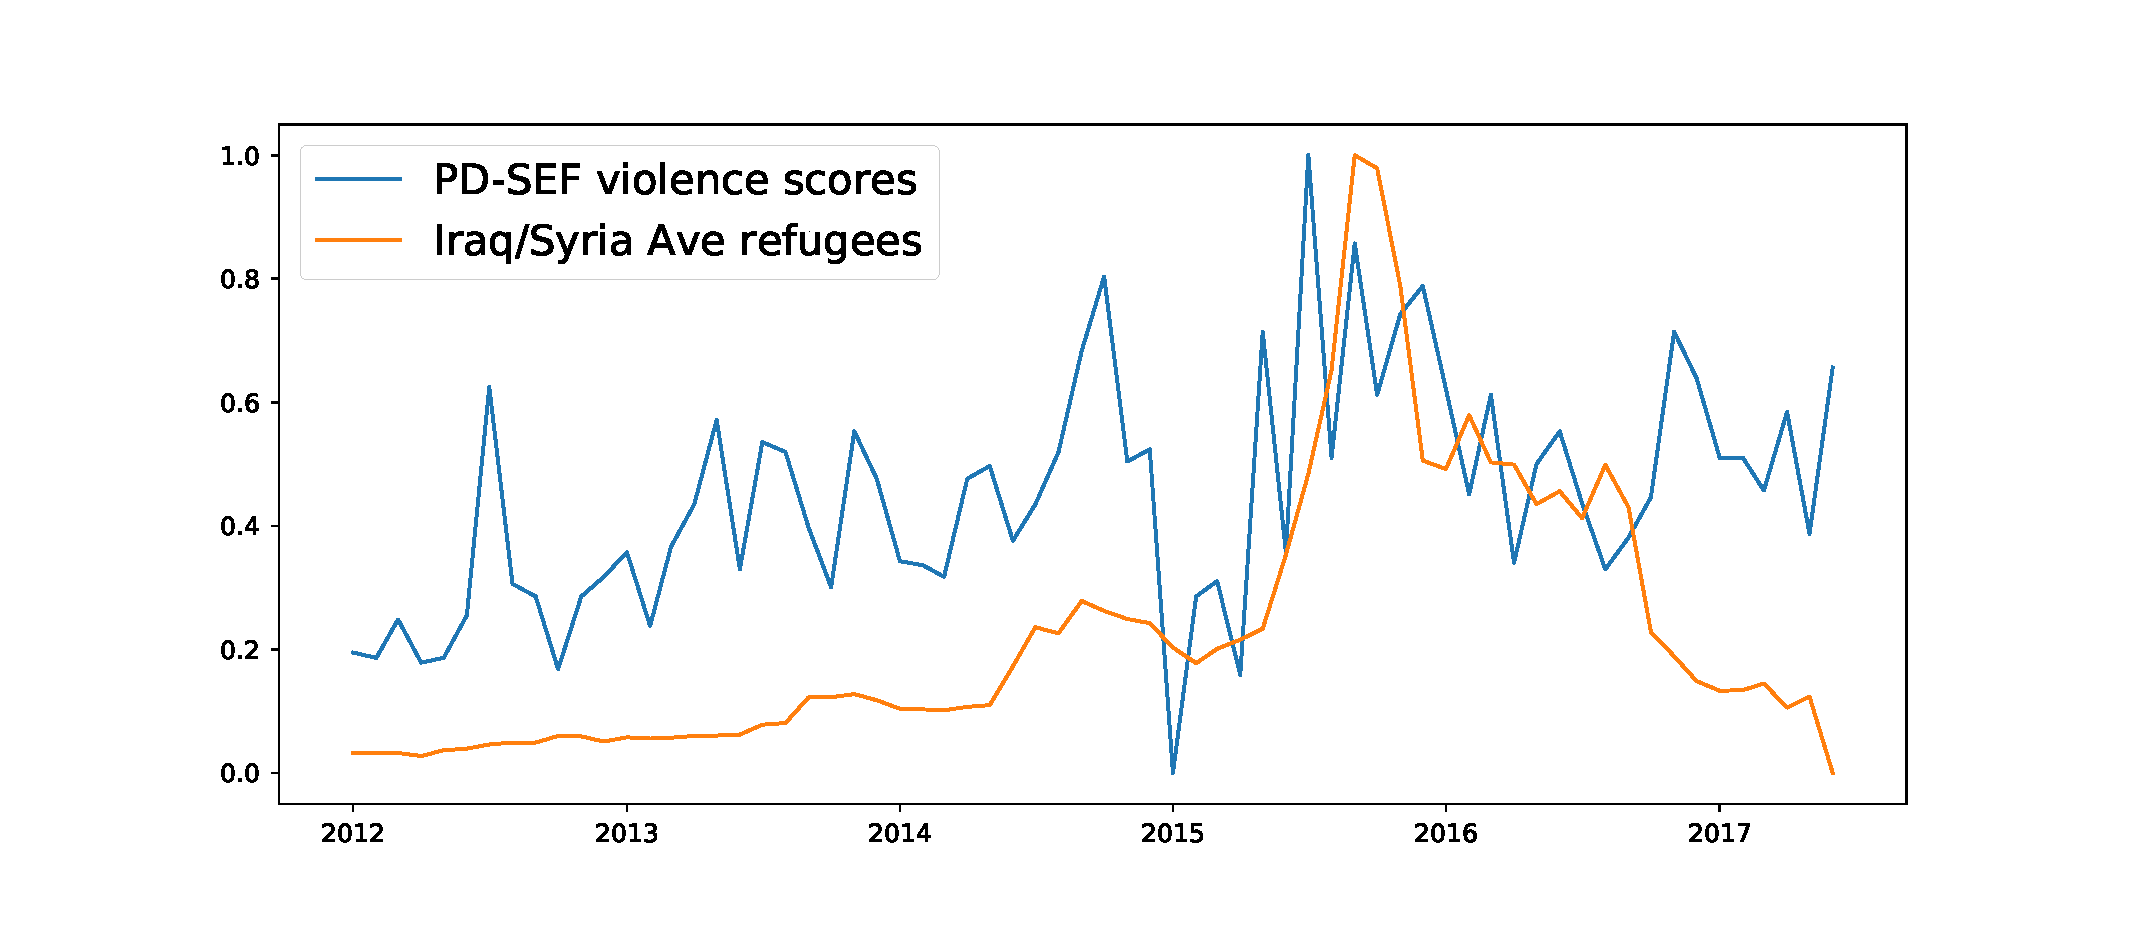
\includegraphics[height=0.55\columnwidth,width=0.9\columnwidth]{img/234.eps}
\end{figure}

Figure \ref{fig:ours} shows PD-SEF violence scores against average refugee population of Iraq and Syria. The PD-SEF is capable of capturing the high trend of violence during 2015 which may have caused the mass population displacement during this year. Furthermore, there is a two months gap between the peak of PD-SEF violence and the peak of population displacement. Removing the gap increases the Pearson correlation from 0.483 to 0.544, validating the assumption that two months is reasonable amount of time between when the triggers of forced migration are observed and when the displacement actually takes place for a large number of people.

\subsection{Classification Evaluation}
Different classification methods are used to classify the topics, including Support Vector Classifier, XGBoost, linear regressions, and Stochastic Gradient Decent. We used 10 fold class validation to measure the performance of the classifiers. Table \ref{tab:classificationresults} reports the best performance of the aforementioned classification methods in terms of precision, recall and F1 score. Values of the parameters of the aforementioned methods, resulting in best performance is described below.
\begin{itemize}
\item SVC: Kernel=linear,
\item SGD: hinge loss function with l2 regularization
\item Logistic Regression: l2 regularization
\end{itemize}
With the choice of best features the performance of classification has considerably improved.
Experiments reveal that SGD classifier performs the best comparing to other classifiers. We are representing our topic documents with the top 50 words in terms of the probability of observing them in the topic. This results shows that the features we extracted from the unlabeled news media through topic modeling are suitable for representing the overall latent space of the corpus. Further, we rely on the classification task to provide automatic label for the population displacement signals from the news media. 

\begin{table}[!ht]
  \centering
  \caption{Topic classification results}
  \label{tab:classificationresults}
%   \resizebox{\textwidth}{!}{
  \begin{tabular}{lccc}
    \toprule
%     Command &A Number & Comments\\
    Classifier & Precision & Recall & F1 Score \\
    \midrule
    SVM (linear) + BOW                             & 0.819     & 0.818  & 0.818    \\ 
    SVM (linear) + TF-IDF                          & \textbf{0.847}     & 0.844  & 0.844    \\ 
    SVM (linear) + GloVe                           & 0.839     & 0.838  & 0.837    \\ 
    \midrule
    XGBoost Classifier + BOW               & 0.825     & 0.825  & 0.825    \\ 
    XGBoost Classifier + TF-IDF            & 0.812     & 0.812  & 0.811    \\ 
    XGBoost Classifier + GloVe             & 0.840     & 0.838  & 0.838    \\ 
    \midrule
    Logistic Regression + BOW              & 0.827     & 0.826  & 0.826    \\ 
    Logistic Regression + TF-IDF           & 0.840     & 0.838  & 0.838    \\ 
    Logistic Regression + GloVe            & 0.841     & 0.840  & 0.840    \\ 
    \midrule
    SGD Classifier + BOW                  & 0.810     & 0.809  & 0.809    \\ 
    SGD Classifier + TF-IDF               & 0.848     & \textbf{0.847}  & \textbf{0.847}    \\ 
    SGD Classifier + GloVe                & 0.844     & 0.843  & 0.843    \\ 
    \midrule
    \bottomrule
  \end{tabular}
%   }
\end{table}



\subsection{Topic Modeling Evaluation}

First, we choose a range of topic numbers for the topic models. In this case, we choose $k$ to be a range between 10 to 30, with increments of two, that is $k \in \{10, 30\}$. Next, the Latent Dirichlet allocation (LDA) Mallet \footnote{http://mallet.cs.umass.edu/} (Gibbs sampling) and Non-negative Matrix Factorization (NMF) topic models are generated using the window slice of the corpus. LDA Mallet is reported to be a strong baseline for analyzing the performance of the topic models \cite{Greene2016}. The window topic space tend to be sensitive to the local and short bursting topics in the large dataset since the models are trained on the subset of entire corpus. Table \ref{table:topic-example} shows the extracted topics and their corresponding labels.

% \FloatBarrier
\begin{table*}[ht]
  \caption{Topics and keyword representation.}
  \label{table:topic-example}

  \resizebox{\textwidth}{!}{%
  \begin{tabular}{l|l}
    \toprule
    Topic label & Top ten words (Sorted by the probability of the word in the topic) \\
    \midrule
    Violence/Terrorism & killed, Baghdad, wound, car, attack, bomb, people, suicide, police, security\\
    Refugee Crisis& refugee, child, million, Jordan, UNHCR, Syrian\_refugee, humanitarian, people, flee, aid \\
    Economical Issues & oil, barrel, export, crude, company, market, energy, price, sanction, say \\
    Political Issues & talk, Istanbul, round, Baghdad, Iran, meeting, Jalili, negotiation, p5, Tehran \\
    \bottomrule
  \end{tabular}
  }
\end{table*}

% \FloatBarrier

\begin{figure}[!ht]
\centering
\captionof{figure}{Topic modeling coherence score}
\label{fig:topic_coherence}
\begin{minipage}{.5\linewidth}
  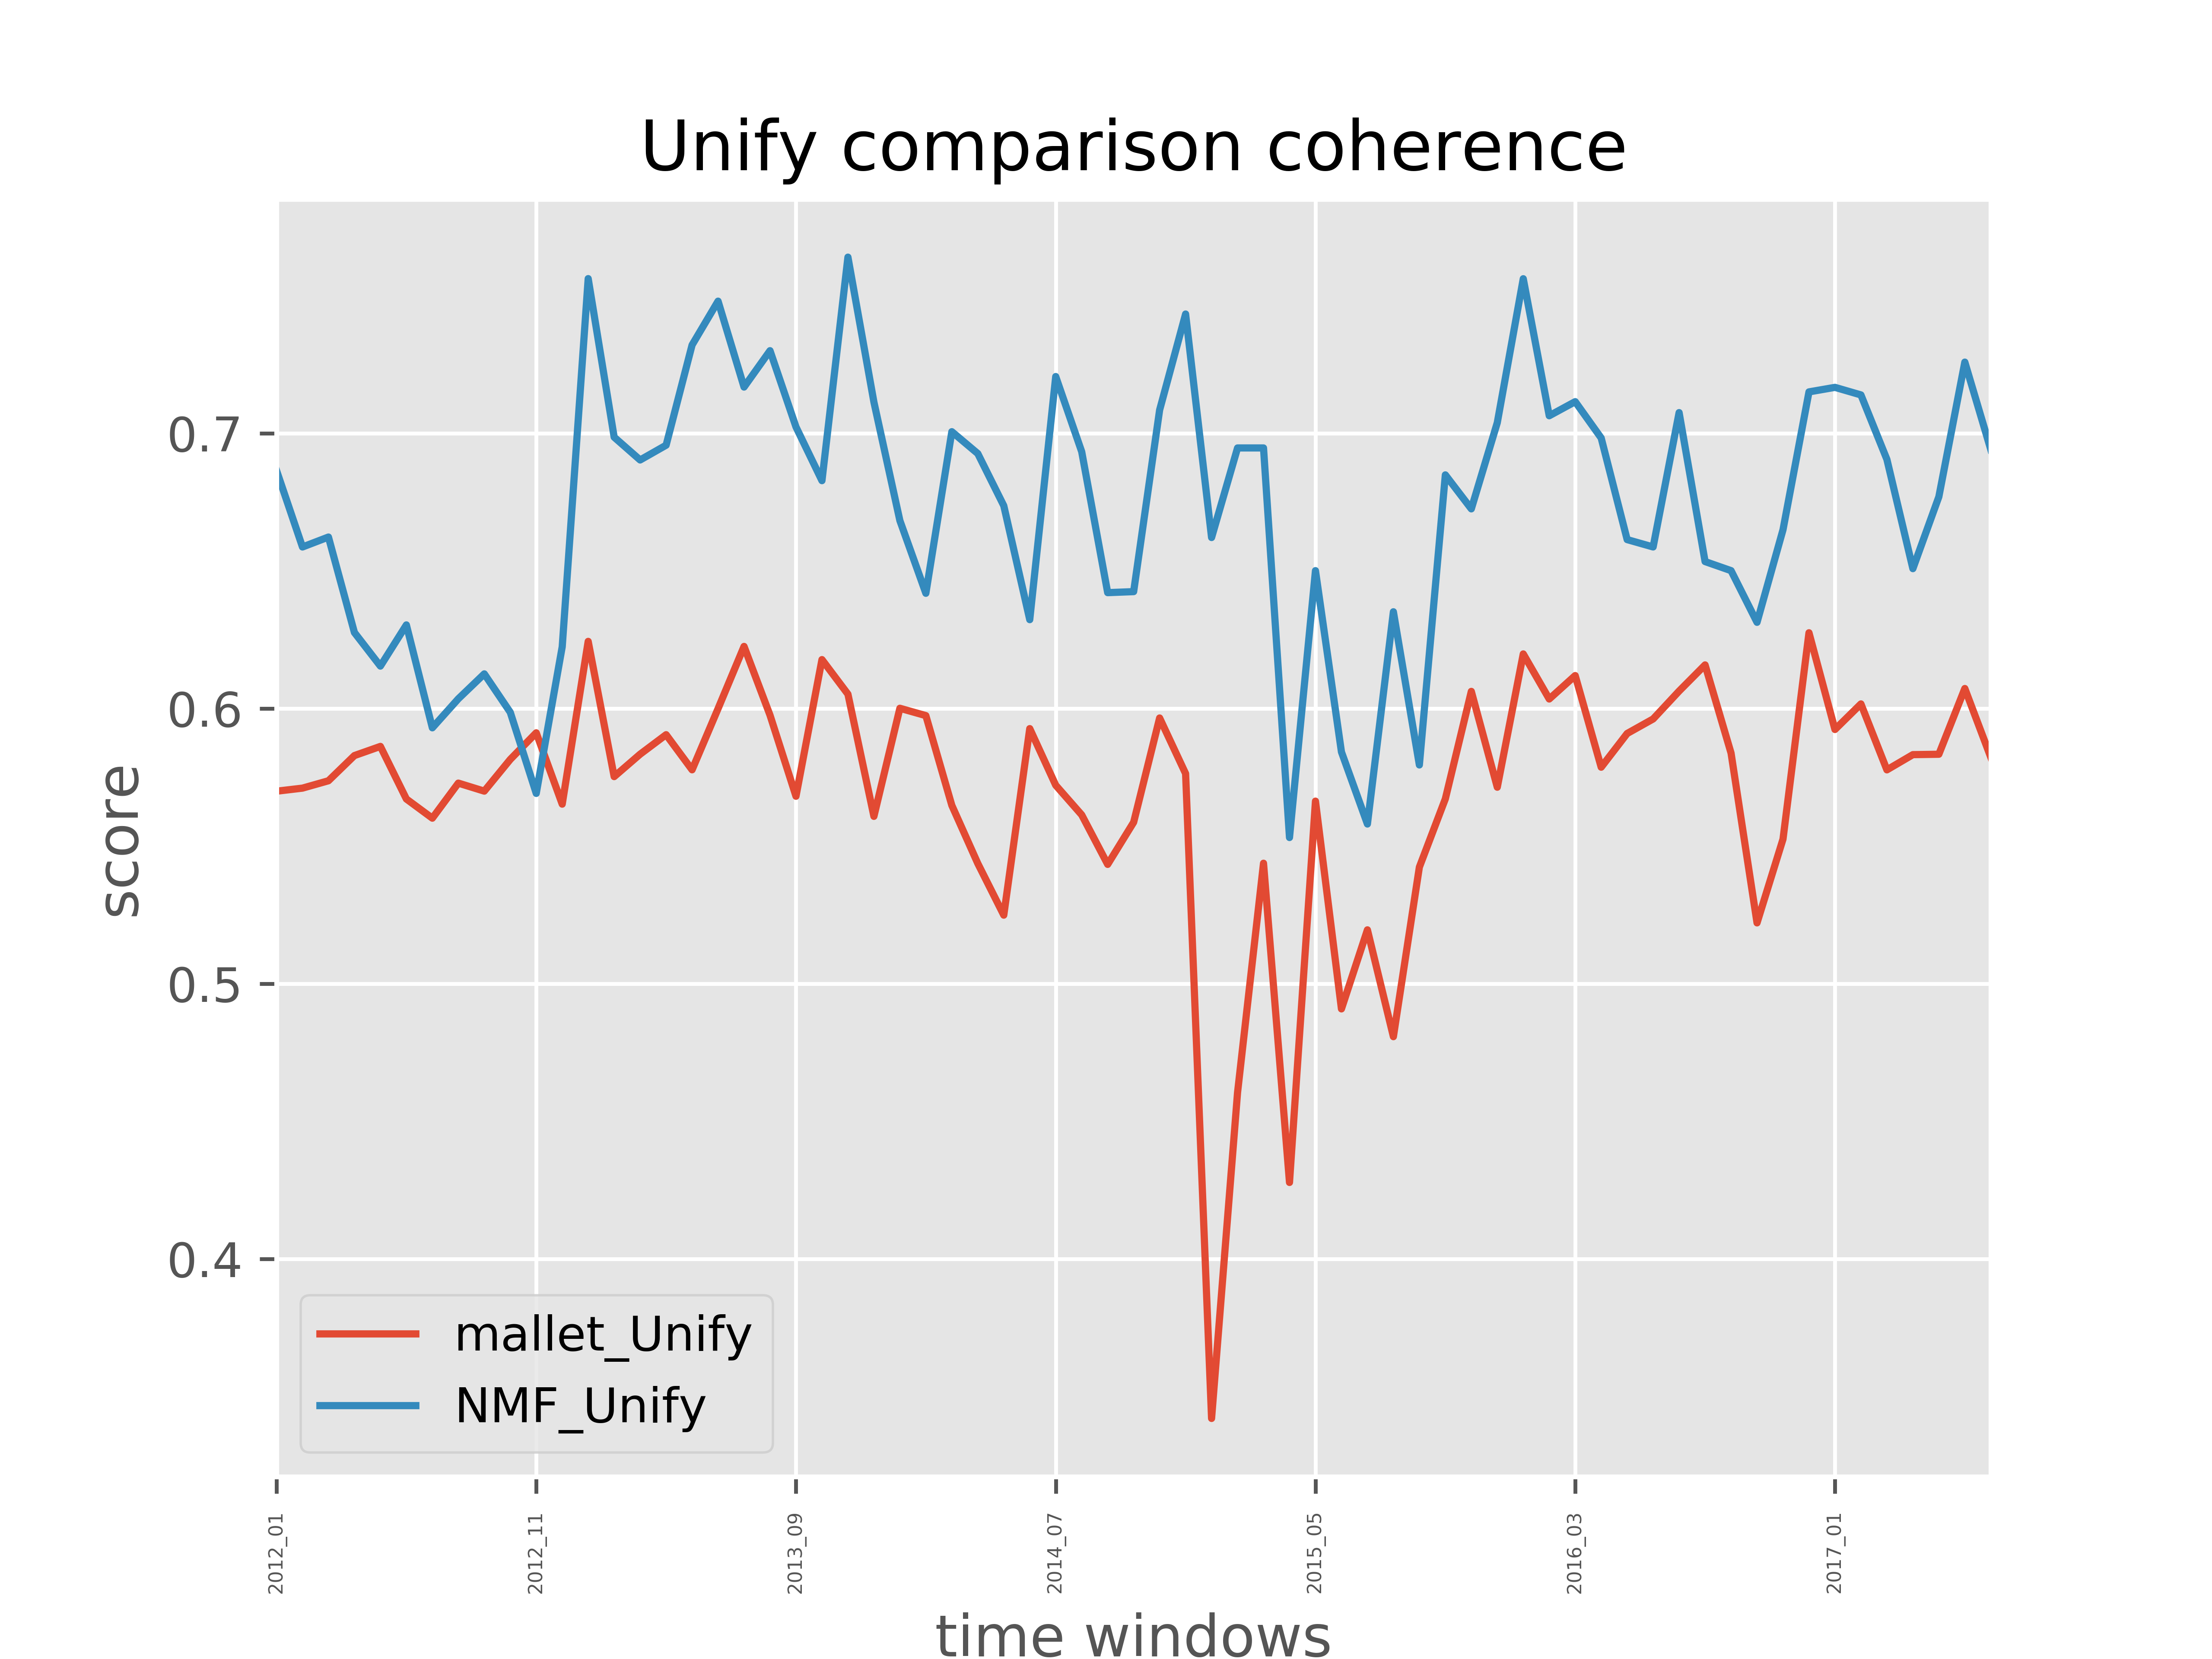
\includegraphics[width=\textwidth]{img/Unify_comparison_all_coherence_plot}
\end{minipage}\hfill
% \hspace{.05\linewidth}
\begin{minipage}{.5\linewidth}
  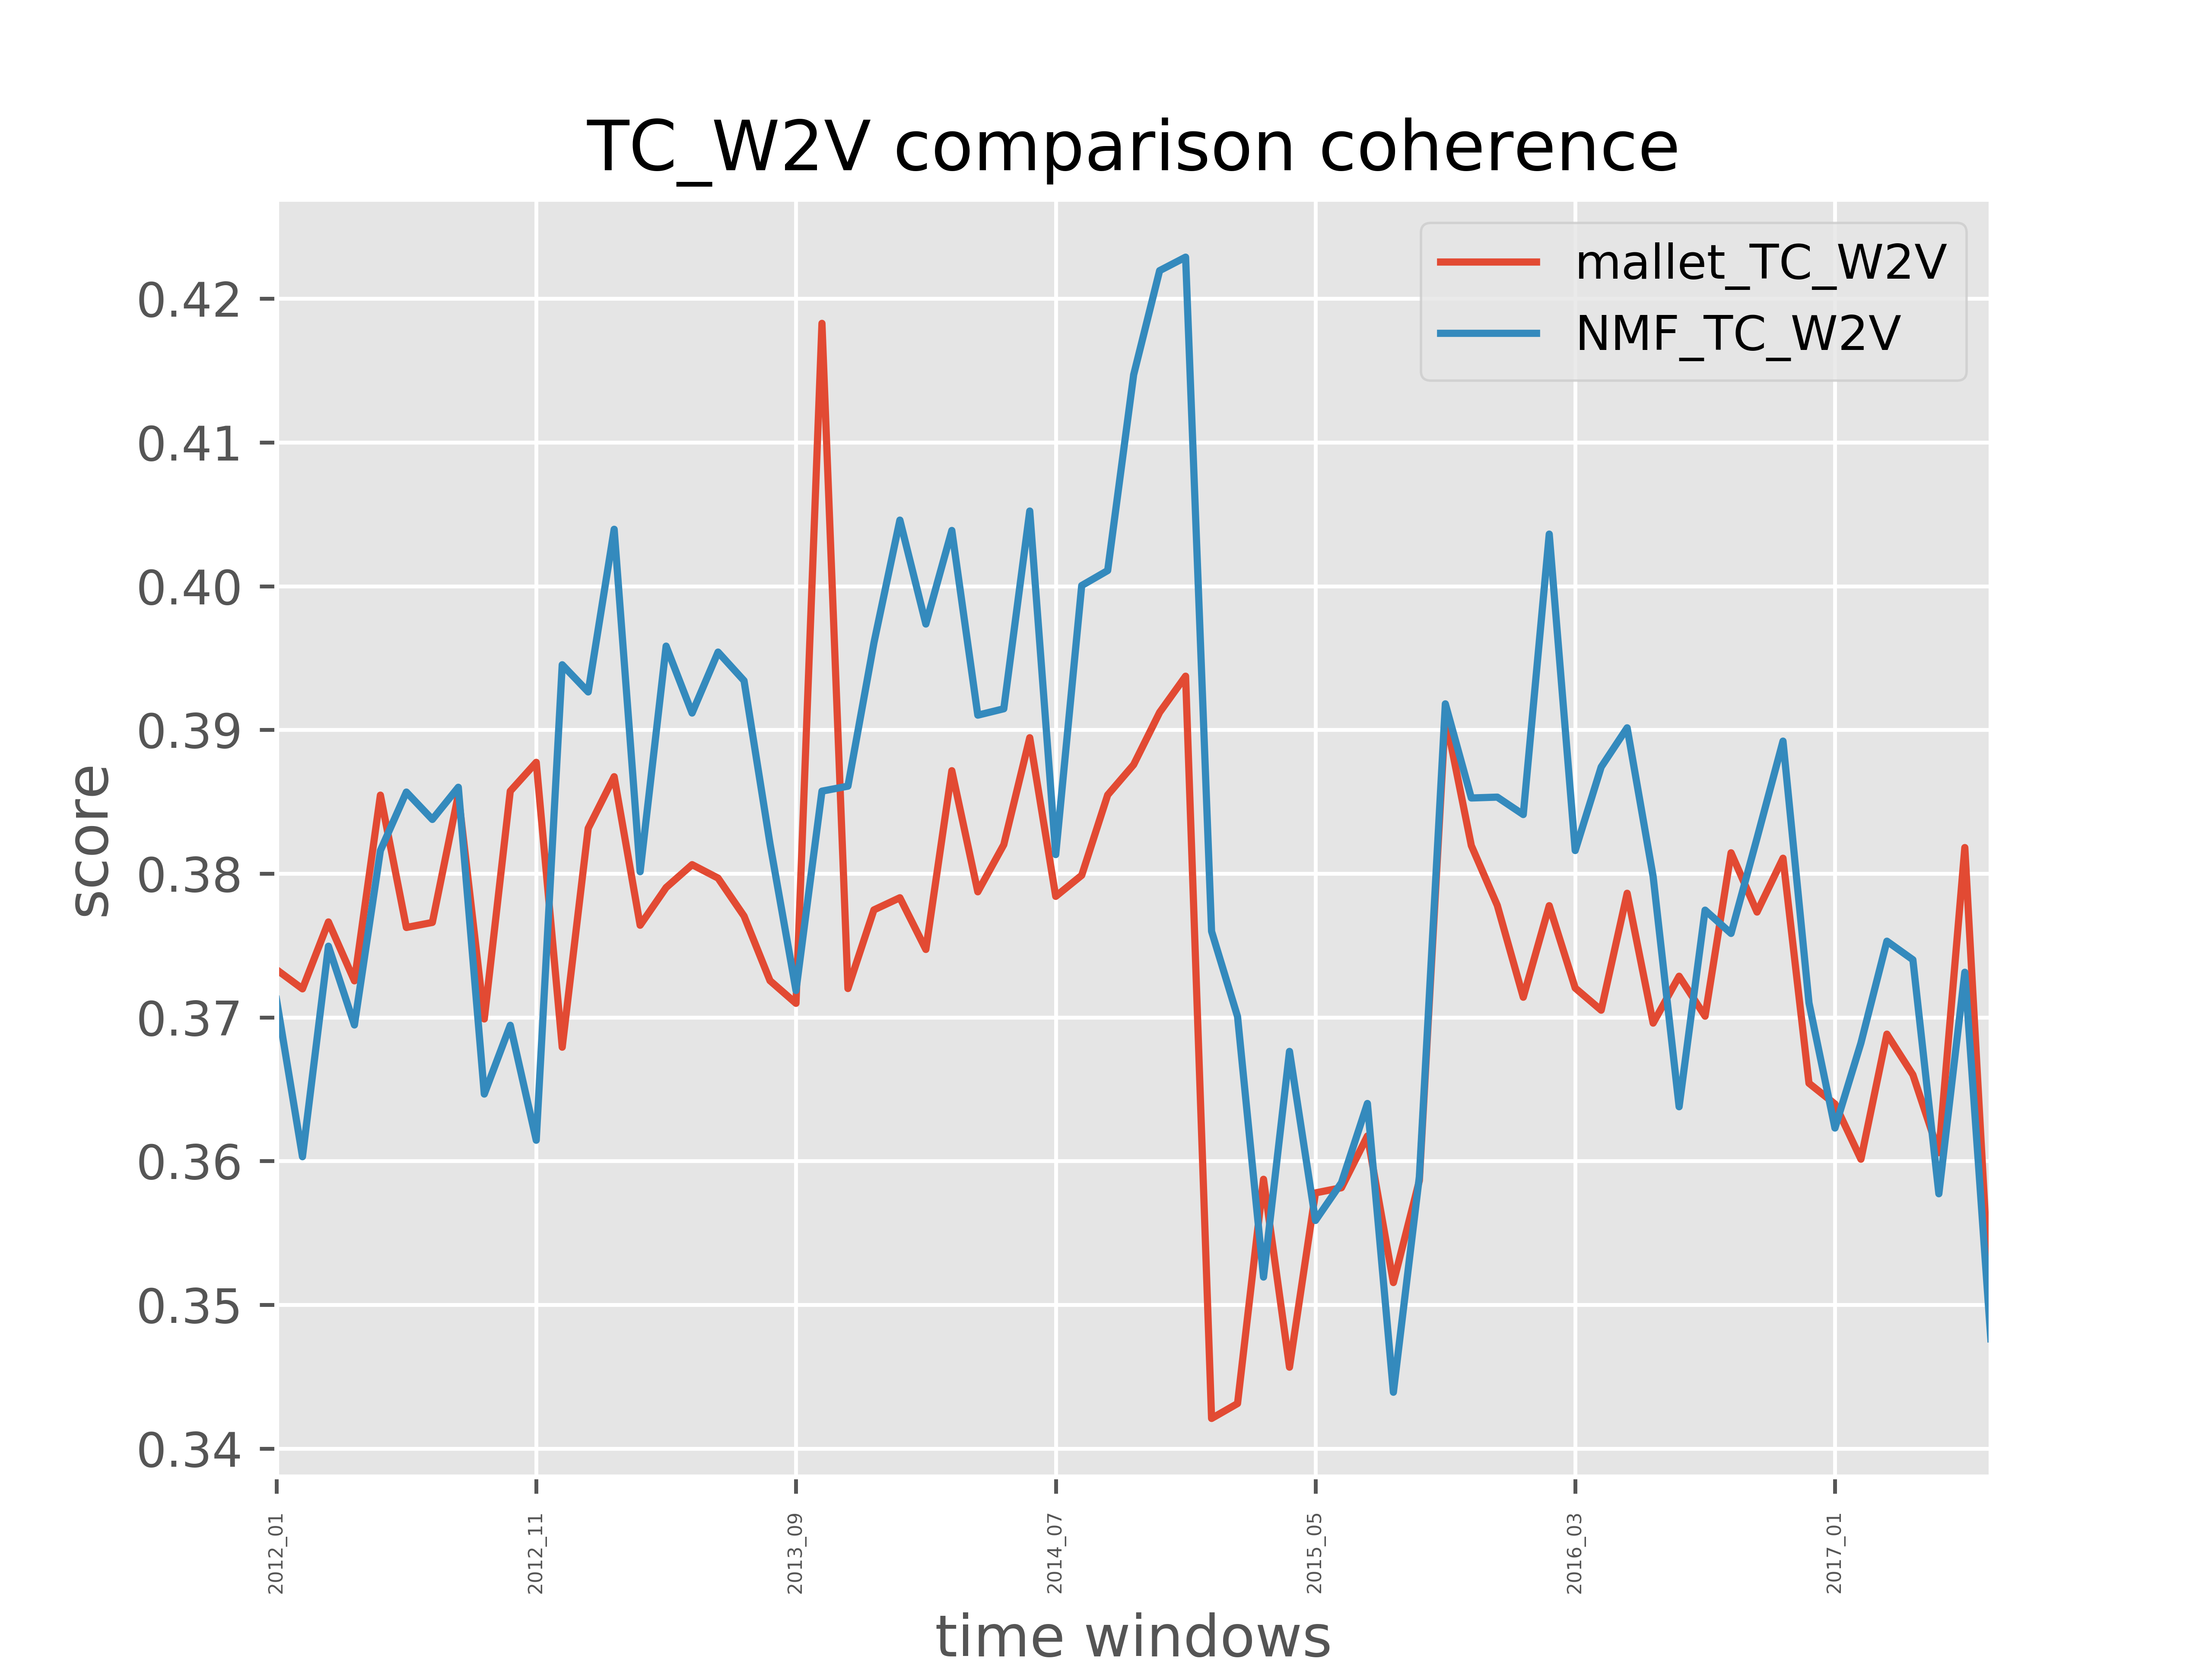
\includegraphics[width=\textwidth]{img/TC_W2V_comparison_all_coherence_plot}
\end{minipage}
\end{figure}

We observed that the NMF topic modeling shows improvements in the topic modeling coherence scores (Fig \ref{fig:topic_coherence}). This result is in agreements with the results discovered in \cite{Greene2016}. Another significant advantage of the NMF, compare to the probabilistic approaches, is the speed of finding topics. The matrix factorization tends to be faster than its counterpart probabilistic based approaches.  


\section{Analysis and Conclusions}
In this paper, we proposed a novel framework (PD-SEF) for processing and analyzing news articles to extract the signals of forced migration and use them to build prediction models for forecasting future displacements. Experiments demonstrated that violence scores are effective features that feeding them to prediction models improves the performance of the models.

The performance of PD-SEF depends on the quality of the news articles such as complete and accurate coverage of the events. Unfortunately, EOS dataset has many missing articles during the first six months of 2015, resulting in negative impact on the quality of our model. This is observable in the sudden drop down in violence scores extracted by PD-SEF during 2015. We believe PD-SEF will show more accurate results using a dataset with better coverage.
Also, there are many other factors affecting refugee migration which might not be extractable from news articles using PD-SEF, such as European Union's policy on accepting more refugees from middle east during 2015 resulting in the significant increase in the number of refugees during this year.

At last, the nature of forced population movement is multi-variant, and therefore it is challenging to establish coherent ground truth for validating our topics and predictions. We did not expect a high degree of correlation between our topics and the refugee movements. This is attributed to the lack of transparent data on the number, causes, and origins of population movements. Also, we realize that the monthly analysis of the news articles provides a limited degree of spatio-temporal awareness, which can't be directly correlated to any related dataset.